\chapter{Desenvolvimento e Análise dos Resultados Obtidos}

Neste capítulo será discutido o que foi efetivamente feito para realização da solução proposta no capítulo 4, assim como a concretização da metodologia utilizada. Também são apresentadas as tecnologias utilizadas e problemas encontrados.

As etapas de desenvolvimento foram:

\begin{enumerate}
    \item Preparação dos dados
    \item Treinamento do modelo de detecção de placas
    \item Implementação do algoritmo de extração de caracteres
    \item Criação dos \textit{datasets} de caracteres e de placas
    \item Treinamento dos modelos de classificação de caracteres
    \item Quantização e transformação dos modelos para formato compatível com o \textit{hardware}
    \item Preparação do \textit{hardware}
    \item Realização dos testes
\end{enumerate}

\section{Preparação dos dados}

O primeiro passo da preparação dos dados foi a separação em conjuntos de treino, validação e teste, cada qual com um propósito diferente: 

\begin{itemize}
    \item \textbf{Treino:} O conjunto de treino é utilizado para ajustar os modelos, que irão se adaptar para minimizar o erro de inferência nesses dados. 
    \item \textbf{Validação:} Este conjunto é utilizado para, durante o treinamento dos modelos, garantir que o ajuste feito com os dados de treino se generalizam para dados não utilizados no treinamento.
    \item \textbf{Teste:} Estes dados não são utilizados em nenhum momento durante o desenvolvimento e ajustes dos modelos. Sua função é serem utilizados nos testes finais para verificar a eficácia do modelo desenvolvido.
\end{itemize}

O \textit{dataset} original continha 10 mil imagens de carros, sendo que destas 5 mil eram com placas do tipo Brasil e 5 mil do tipo Mercosul. Os dados foram então divididos da seguinte forma: 70\% para o conjunto de treino, 20\% para o conjunto de validação e 10\% para o conjunto de teste. Os dados colocados em cada conjunto foram selecionados aleatoriamente, mas garantindo que cada conjunto teria 50\% de imagens com placas Mercosul e 50\% com placas Brasil.

\subsection{Organização dos dados}

O treinamento do modelo de detecção de placas foi realizado com a biblioteca Ultralytics do python. Essa biblioteca, além de oferecer diversos modelo da família YOLO, já inclui o algoritmo de treinamento, necessitando apenas que o usuário deixe os dados organizados em um formato específico. Esse formato inclui deixar os dados de treino e validação em pastas separadas, além de escrever os arquivos de anotações em um formato específico.

Os arquivos de anotações são os arquivos que contém as informações das \textit{bounding boxes} e pontos-chave das imagens. O Ultralytics exige que eles sejam arquivos do tipo txt com o mesmo nome do arquivo de imagem ao qual se referem. Por exemplo, a imagem $img\_000001.jpg$ deve ter um arquivo $img\_000001.txt$ correspondente que contém as anotações daquela imagem.

O arquivo de anotações pode ter múltiplas linhas, cada um correspondendo a um objeto na imagem. Cada linha é composta da seguinte forma:

\begin{verbatim}
<classe> <x centro> <y centro> <largura> <altura> <x ponto 1> 
<y ponto 1> <visibilidade ponto 1> ... <x ponto n> <y ponto n> 
<visibilidade ponto n>
\end{verbatim}

A classe é o número da classe daquele objeto. No caso do projeto existem duas classes: placa Brasil (0) e placa Mercosul (1). O $x \; centro$ e $y \; centro$ correspondem às coordenadas $(x,y)$ do centro do objeto. A largura e altura, como o nome sugere, são a largura e altura do objeto. Por fim, cada ponto-chave é composto por três informações: coordenada $x$, coordenada $y$ e visibilidade. Como em todas as imagens a placa está com os quatro cantos visíveis, a visibilidade é sempre 2, que é o valor que representa pontos visíveis. Toda sas coordenadas, assim como altura e largura são normalizadas para que fiquem entre 0 e 1.

\section{Treinamento do modelo de detecção de placas}

Com os dados preparados nas pastas, basta criar um arquivo de configuração no format YAML e escrever um simples script em python para iniciar o treinamento do modelo desejado. O arquivo de configuração deve conter as seguintes especificações:

\begin{itemize}
    \item O caminho para a pasta que contém os dados
    \item O sub caminho para as pastas que contém os dados de treino e validação
    \item O número de classes
    \item Os nomes das classes
    \item O formato dos pontos-chave
    \item Índice espelhado dos pontos-chave
\end{itemize}

No caso deste projeto o número de classes é 2, cujos nomes foram definidos como \textit{placa\_br} e \textit{placa\_me}. O formato dos pontos-chave deve ser uma tupla contendo dois valores: O número de pontos-chave por objeto e a dimensão dos pontos-chave, que é 3 (largura, altura, visibilidade). O índice espelhado dos pontos-chave é uma lista de índices de 0 a n sendo que n é a quantidade de pontos-chave por objeto. A ordenação dos índices deve indicar como os índices devem ser tratados caso a imagem seja espelhada horizontalmente. Isso é necessário pois o Ultralytics faz isso com algumas imagens durante o processo de treinamento.

Com o arquivo de configuração preparado é possível executar o script de treinamento, que é bastante simples. Precisa primeiro importar a biblioteca Ultralytics e criar um objeto da classe YOLO, que recebe como argumento o nome do modelo YOLO desejado, que no caso é \textit{yolo26n-pose}. Em seguida basta chamar o método \textit{train}, indicando o caminho para o arquivo de configuração que foi criado, o tamanho do \textit{batch} desejado, o número de épocas e o dispositivo no qual executar o modelo.

Foram treinadas 100 épocas no dispositivo \textit{cuda} (GPU do computador). O tamanho do \textit{batch} foi deixado como -1, que faz com que o próprio Ultralytics defina o melhor tamanho de \textit{batch} com base na capacidade da GPU. As 100 épocas se mostraram suficientes para ajustar o modelo, que ao final do treinamento estava com um erro bem pequeno e estável, tanto na detecção dos objetos como na classificação e detecção dos pontos-chave.

A figura \ref{fig:yolotrain} mostra três curvas do erro do modelo ao longo do treinamento. A primeira é o erro do ajuste da \textit{bounding box}, a segunda é o erro dos pontos-chave e a terceira é o erro de classificação.

\begin{figure}[H]
    \centering
    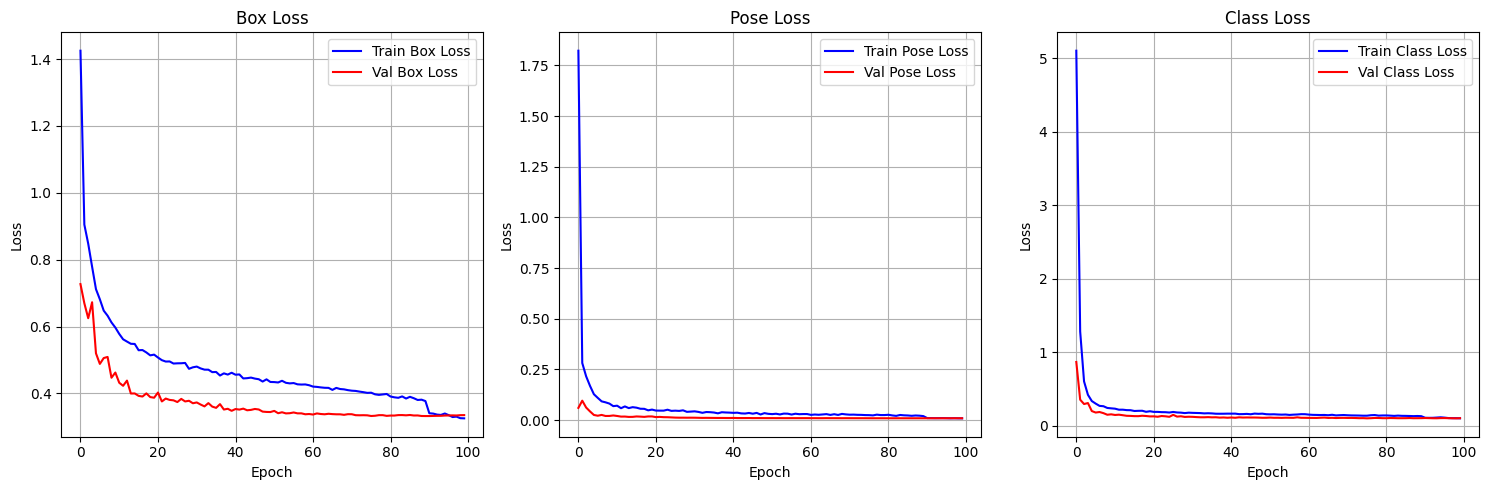
\includegraphics[width=1.0\linewidth]{images/yolo-train.png}
    \caption{Curvas de treinamento do modelo de detecção de placas}
    \label{fig:yolotrain}
\end{figure}

\subsection{Exportação do modelo YOLO}

Findado o treinamento o Ultralytics automaticamente exporta um arquivo com os pesos do modelo ajustados. Porém esse formato é compatível apenas para realizar inferência com a própria biblioteca Ultralytics. Para obter o modelo em um formato com mais portabilidade, basta criar um novo script, carregar o modelo treinado e utilizar o método \textit{export} para obter o modelo em um arquivo do tipo ONNX. Esse formato permite inferência em diversas plataformas através da biblioteca \textit{onnx runtime}, mas também permite que o modelo seja carregado pelo software que realiza a conversão para o formato RKNN, compatível com a NPU da placa Rock 3A.

\section{Implementação do algoritmo de extração de caracteres}

Após o ajuste do modelo de detecção de placas, foi criado o script de processamento das imagens e extração dos caracteres. Esse script foi feito em python, e utilizou a biblioteca \textit{onnx runtime} para realizar inferência com o modelo de detecção de placas exportado para formato ONNX.

As etapas do script são as seguintes:

\begin{enumerate}
    \item Inferência com o modelo de detecção de placas
    \item Criação de uma nova imagem contendo apenas a placa, cortada da imagem original com base na \textit{bounding box} gerada pelo modelo de detecção
    \item Correção de perspectiva
    \item Remoção das bordas da placa com base no tipo de placa verificado pelo modelo de detecção
    \item Binarização da imagem
    \item Separação dos caracteres
    \item Limpeza das imagens dos caracteres
\end{enumerate}

A seguir será discutida em mais detalhes a implementação de cada etapa do script.

\subsection{Inferência com o modelo de detecção de placas}

O modelo YOLO foi treinado com a biblioteca Ultralytics e exportado para formato ONNX, podendo agora ser utilizado para inferência com a biblioteca do python \textit{onnx runtime}. A implementação da inferência, então, incluiu carregar o arquivo do modelo e criar uma função que recebe a imagem e devolve a inferência.

A função não se limita simplesmente a alimentar a imagem ao modelo, pois é necessário algum pré-processamento da imagem antes disso. Primeiramente a imagem deve ser redimensionada para o formato $640 \times 640$ px, que é a dimensão utilizada pelo YOLO. Em seguida os valores dos pixels devem ser normalizados para que fiquem entre 0 e 1.

O redimensionamento foi feito com a biblioteca de manipulação de imagens OpenCV, assim como o próprio carregamento da imagem. O OpenCV carrega a imagem como um tensor de dimensão (H,W,C), onde H é a altura da imagem, W é a largura e C é o número de canais, que é 3 para imagens coloridas e 1 para imagens em escala de cinza. Cada valor representa a intensidade de um pixel em um dado canal (para imagens coloridas os canais são vermelho, verde, azul), que é representada por um número inteiro de 0 a 255 (8 \textit{bits}).

O OpenCV oferece uma função para redimensionamento de imagem, já a normalização pode ser feito simplesmente dividindo o tensor por 255. Com isso, a imagem fica pronta para ser alimentada ao modelo.

A última etapa dessa implementação é a interpretação da saída do modelo. Ao alimentar o modelo com a imagem, ele devolve uma saída no formato de uma matriz $300x18$. Cada linha dessa matriz representa uma detecção representada por 18 valores. A única detecção que nos interessa é a primeira, pois as detecções são ordenadas em ordem de confiança. O modelo é obrigado a gerar 300 detecções pela forma como foi construído, mas a maioria delas não representa nenhum objeto. Como nosso objetivo é analisar apenas uma placa por imagem, pegamos apenas a primeira detecção e descartamos as demais, de forma que se houver mais de uma placa, apenas a mais visível será analisada.

Dos 18 valores que representam a detecção a interpretação é a seguinte:

\begin{itemize}
    \item Os 4 primeiros valores representam a \textit{bounding box} do objeto na seguinte ordem: $x_1,y_1,x_2,y_2$
    \item O quinto valor representa a confiança da detecção, que vai de 0 a 1
    \item A classe do objeto (\textit{placa\_br} ou \textit{placa\_me}) é representada pelo sexto valor
    \item As coordenadas dos pontos-chave são os valores seguintes
\end{itemize}

Como a imagem foi redimensionada para $640 \times 640$ é necessário converter as coordenadas dos pontos-chave e da \textit{bounding box} para a dimensão da imagem original. Para isso basta multiplicar as coordenadas $x$ pela largura da imagem original e as coordenadas $y$ pela altura e dividir todas por por 640. Assim temos as coordenadas nas dimensões da imagem original.

\subsection{Criação de nova imagem contendo apenas a placa}

Com base na \textit{bounding box} gerada pelo modelo, é possível cortar a imagem original e gerar uma imagem que contenha apenas a placa detectada. Antes disso, porém, convertemos a imagem para escala de cinza, de forma que seja representada por uma única matriz (H x W). A conversão para escala de cinza é feita pela biblioteca OpenCV.

Depois disso, basta criar uma nova matriz apenas com os pixels cujas coordenadas $(x,y)$ obedecem às limitações: $x_1 \le x \le x_2$ e $y_1 \le y \le y_2$, sendo que $x_1,x_2,y_1,y_2$ são os limites da \textit{bounding box} na imagem original.

\subsection{Correção de perspectiva}

A correção de perspectiva é realizada pela biblioteca OpenCV em uma sequência de etapas:

\begin{enumerate}
    \item Definição das coordenadas dos pontos antes da transformação
    \item Definição das coordenadas dos pontos depois da transformação
    \item Geração da matriz de transformação
    \item Transformação com base na imagem e na matriz
\end{enumerate}

Os pontos antes da transformação nada mais são do que as coordenadas dos pontos-chave encontrados pelo YOLO. A única questão é que eles precisam ser transformados para que a referência das coordenadas seja a imagem cortada, não a imagem original. A operação para essa transformação foi discutida no capítulo 4.

Os pontos pós transformação nada mais são que os quatro cantos de uma imagem hipotética de dimensões $W_2 \times H_2$. Essa dimensão será a dimensão da imagem após a transformação, que foi definida como $500 \times 200$. Portanto os 4 pontos pós transformação são: $(0,0)$, $(499,0)$, $(499,199)$, $(0,199)$.

Definidos os pontos pode ser gerada a matriz de transformação com base neles, o que é feito através de uma função do OpenCV. Em seguida, basta utilizar uma outra função do OpeCV para obter a imagem transformada com base na matriz de transformação, na imagem inicial (imagem cortada da placa) e nas dimensões desejadas da imagem final.

Com isso, temos uma função que recebe uma imagem com dimensões $(w \times h)$ de uma placa e o \textit{output} do modelo YOLO e devolve uma imagem de dimensões $(500 \times 200)$ com a perspectiva da placa corrigida.

\subsection{Remoção das bordas das placas e binarização}

A remoção das bordas das placas implica basicamente em cortar as imagens de acordo com as dimensões do tipo de placa. Para fazer isso basta limitar os pixels que devem fazer parte da imagem cortada. Considerando as coordenadas $(x,y)$ dos pixels basta seguir o padrão:

\begin{gather}
    c_l \le x \le 500 - c_r \\
    c_t \le y \le 200 - c_b
\end{gather}

Sendo que $c_l$, $c_r$, $c_t$ e $c_b$ são a quantidade de pixels a cortar na esquerda, direita, topo e parte de baixo da imagem, respectivamente. Esses valores são diferentes para placas do tipo Brasil e Mercosul, como discutido no capítulo 4.

A binarização, que utilizou o método de Sauvola, foi feita utilizando algumas funções diferentes do OpenCV. O primeiro passo foi gerar uma imagem na qual cada pixel era a média dos pixels vizinhos na imagem da placa. Para isso, foi utilizada uma função do OpenCV que faz exatamente essa tarefa a partir de uma imagem e um tamanho de janela, que para o nosso caso foi escolhido 201 pixels. Esse é um tamanho relativamente grande considerando que a imagem possui 500 pixels de largura, mas o propósito é justamente não permitir flutuação demais para que o resultado seja menos afetado por ruído e capture apenas a variação de luminosidade ao longo da imagem.

Em seguida foi calculado a mesma coisa para o quadrado da imagem (a intensidade de cada pixel foi elevada ao quadrado). Por fim, utilizando simples operações matemáticas, foi calculado o limiar para cada pixel da imagem, e foi gerada uma imagem binarizada na qual cada pixel era 0 ou 1, a depender se o pixel da imagem original naquela posição era menor ou maior que o pixel na matriz de limiar para aquela posição.

As equações para calculo da matriz de limiar foram discutidas mais a fundo no capítulo 2.

\subsection{Separação dos caracteres}

A implementação da separação de caracteres da imagem binarizada se baseou na seguinte sequência de eventos:

\begin{enumerate}
    \item É gerada uma estimativa dos pontos de separação, cada uma representada como uma coordenada \textit{x} da imagem da placa
    \item A função itera por cada um desses pontos, tentando encontrar um ponto de divisão melhor nos seus arredores
    \item Os pontos de divisão refinados são utilizados para dividir a imagem em \textit{n} pedaços, cada um contendo apenas um caractere
    \item Cada imagem de caractere é "estampada" em uma imagem preta quadrada
\end{enumerate}

Para funcionar a função precisa dos seguintes parâmetros:

\begin{itemize}
    \item A imagem a ser separada
    \item A quantidade de caracteres presentes naquela imagem
    \item O tamanho da janela na qual um ponto de corte melhor será procurado (padronizado em 40)
\end{itemize}

A quantidade de caracteres presentes na imagem define o número de separações a ser feito. Isso é importante pois enquanto as placas do tipo Mercosul são separadas de uma só vez, as placas do tipo brasil são primeiro divididas em duas para que depois cada parte seja separada, como já discutido no capítulo 4.

O tamanho da janela define a até quantos pixels de distância do ponto de separação inicialmente estimado será buscado um ponto de separação melhor. A avaliação dos candidatos a pontos de separação é simples: Cada ponto é uma coluna da imagem, sendo então somadas a intensidade de todos os pixels naquela coluna. Como a binarização já foi feita, pixels que não pertencem a nenhum caractere possuem valor 0, enquanto os que pertencem possuem valor 1. Portanto, a coluna cuja soma das intensidades dos pixels for menor (idealmente 0) é melhor para a divisão, pois provavelmente é um espaço vazio entre dois caracteres.

Depois de dividir a imagem, porém, cada uma terá uma largura diferente. Isso é então padronizado ao gerar uma imagem quadrada preta $H \times H$ (onde $H$ é a altura da imagem da placa) e "estampando" a imagem com o caractere no meio dessa imagem. Isso garante que todas as imagens de caracteres terão as mesmas dimensões.

\subsection{Limpeza das imagens de caracteres}

Para a limpeza das imagens de caracteres foi utilizada a biblioteca \textit{scikit-image} do Python. Ela oferece uma função que, ao receber uma imagem binarizada, como são as imagens de caracteres, mapeia cada pixel branco (valor 1) como parte de um objeto, com base na continuidade. Todo pixel branco que está adjacente a um outro pixel branco faz parte do mesmo objeto que este. Dessa forma a imagem é dividida em vários objetos, e representada por uma matriz na qual cada pixel é um "rótulo", um valor inteiro que indica a qual objeto pertence. Pixels com valor zero são pixels pretos, portanto não pertencem a objeto nenhum.

O \textit{scikit-image} então oferece uma outra função na qual recebe essa matriz de rótulos e calcula características dos objetos, como altura, largura, área, etc. A única que nos interessa é a área, pois ela é o melhor indicativo de qual é o maior objeto da imagem, que seria o caractere. Com base nisso, então, pixels que não pertencem ao objeto de maior área são eliminados da imagem do caractere, passando a ter valor zero. Isso elimina ruído e deixa a imagem do caractere mais limpa, minimizando a propensão à erros de classificação daquele caractere.

\section{Criação dos \textit{datasets} de caracteres e de placas}

Finalizados todos os algoritmos de processamento das imagens passa a ser possível criar os \textit{datasets} para o treinamento dos modelos de classificação. Como temos duas abordagens distintas de modelos, foram criados dois \textit{datasets}: Um com imagens de caracteres binarizadas e limpas e uma com imagens em escala de cinza de placas com perspectiva corrigida.

Para criar o \textit{dataset} de caracteres todas as imagens do conjunto de treino e validação inicial fora submetidas ao \textit{pipeline} completo desenvolvido até aqui. Passaram pelo modelo YOLO, onde a placa foi detectada, foram cortadas para manter só a imagem da placa, convertidas para escala de cinza, tiveram sua perspectiva corrigida, passaram pela remoção de bordas, binarização, separação de caracteres e limpeza. Ao final de tudo, cada imagem de caractere foi rotulada com o caractere contido naquela imagem, que era sabido pelo fato de termos nos dados originais as informações das placas dos carros contidos neles. Todas as imagens foram então salvas em pastas de acordo com:

\begin{itemize}
    \item O tipo de caractere (número ou letra)
    \item O tipo de placa (Brasil ou Mercosul)
\end{itemize}

Os nomes das imagens salvas foram compostos pelo caractere representado na imagem, o nome da imagem original da qual o caractere foi extraído e a posição do caractere na placa (0 - 6).

O \textit{dataset} de placas teve um processo de criação mais simples. As imagens originais passaram pela detecção, corte, transformação para escala de cinza e correção de perspectiva, apenas. Com isso já se tinham imagens de placas com dimensões padronizadas, que foram então salvas em pastas separadas apenas pelo tipo de placa (Brasil, Mercosul). Os nomes das imagens continham os caracteres da placa e mais um código identificador.

\section{Treinamento dos modelos de classificação de caracteres}

Foram feitos dois treinamentos de modelos de classificação de caracteres. O primeiro de modelos de classificação de caracteres isolados, como os gerados pelo \textit{pipeline} completo de extração de caracteres, e o outro de modelos de extração e classificação, com intenção de classificar os caracteres direto das imagens de placas extraídas e com perspectiva corrigida. Ambos foram realizados utilizando a biblioteca PyTorch e ao final do treinamento exportados para o formato ONNX.

Os treinamentos foram realizados utilizando o seguinte ciclo:

\begin{enumerate}
    \item \textit{Batch} de imagens é alimentado ao modelo
    \item É calculado o \textit{Loss} do \textit{Batch} (\textit{Cross Entropy})
    \item É realizado \textit{backpropagation} para cálculo do gradiente
    \item Os pesos do modelo são atualizados
\end{enumerate}

Esses passos são repetidos até que o modelo tenha sido alimentado com todos os dados do \textit{dataset}. É então finalizada a época, o modelo é avaliado e tudo é feito novamente até que o número de épocas determinado inicialmente seja atingido.

\subsection{Classificação de caracteres isolados}

As características específicas do modelo de classificação de caracteres isolados são os seguintes parâmetros de treinamento:

\begin{itemize}
    \item \textit{Optimizer}: Adam com \textit{learning rate} de 0.001
    \item Tamanho do \textit{batch}: 32
    \item Número de épocas: 10
\end{itemize}

Foram treinados um total de quatro modelos distintos, cada um especializado em um tipo de caractere e um tipo de placa, seguindo a divisão feita na criação do \textit{dataset} de caracteres.

As figuras \ref{fig:menumerostrain}, \ref{fig:meletrastrain}, \ref{fig:brnumerostrain} e \ref{fig:brletrastrain} mostram as curvas do \textit{Loss} de treinamento e validação, além da acurácia de validação de cada modelo ao longo das épocas de treinamento. Esses dados foram coletados ao fim de cada época com intenção de registrar a evolução do modelo ao longo do treinamento.

\begin{figure}[H]
    \centering
    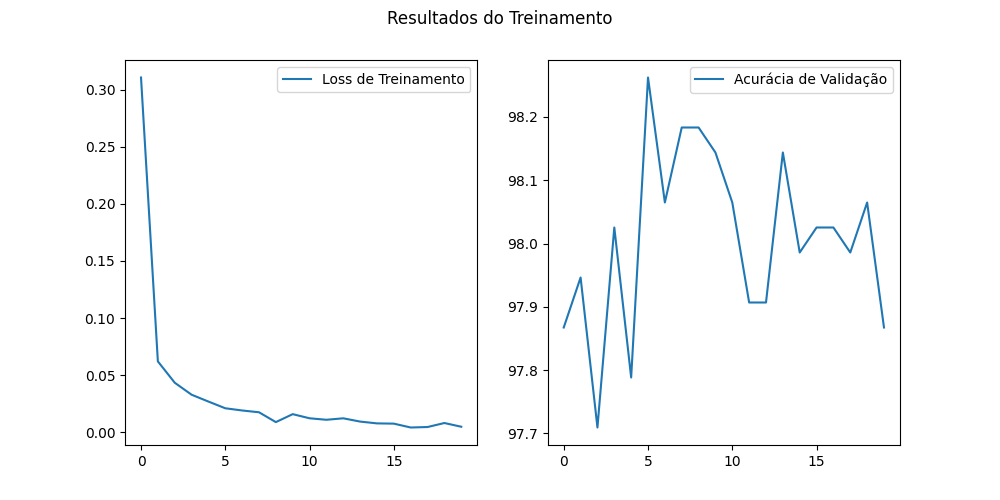
\includegraphics[width=0.8\linewidth]{images/me-numeros.png}
    \caption{Curvas de treinamento do modelo de classificação de números em placas do tipo Mercosul}
    \label{fig:menumerostrain}
\end{figure}

\begin{figure}[H]
    \centering
    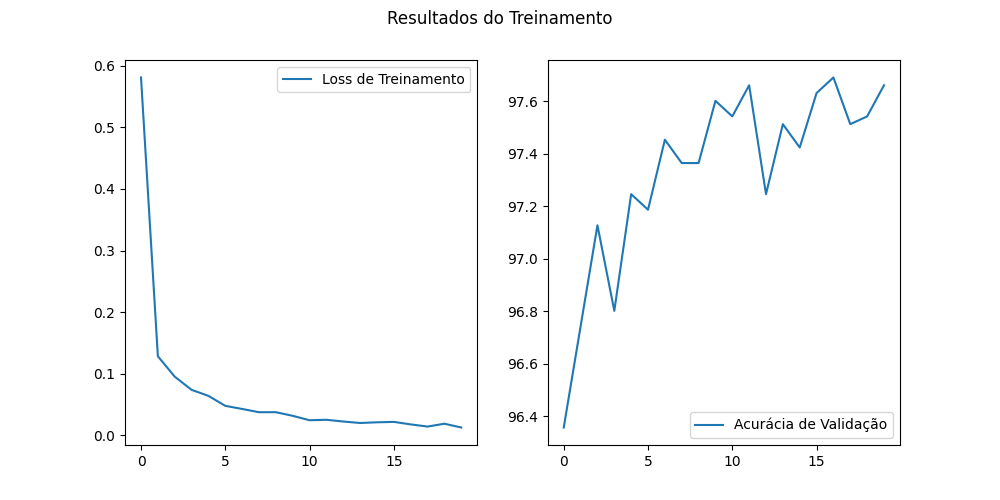
\includegraphics[width=0.8\linewidth]{images/me-letras.png}
    \caption{Curvas de treinamento do modelo de classificação de letras em placas do tipo Mercosul}
    \label{fig:meletrastrain}
\end{figure}

\begin{figure}[H]
    \centering
    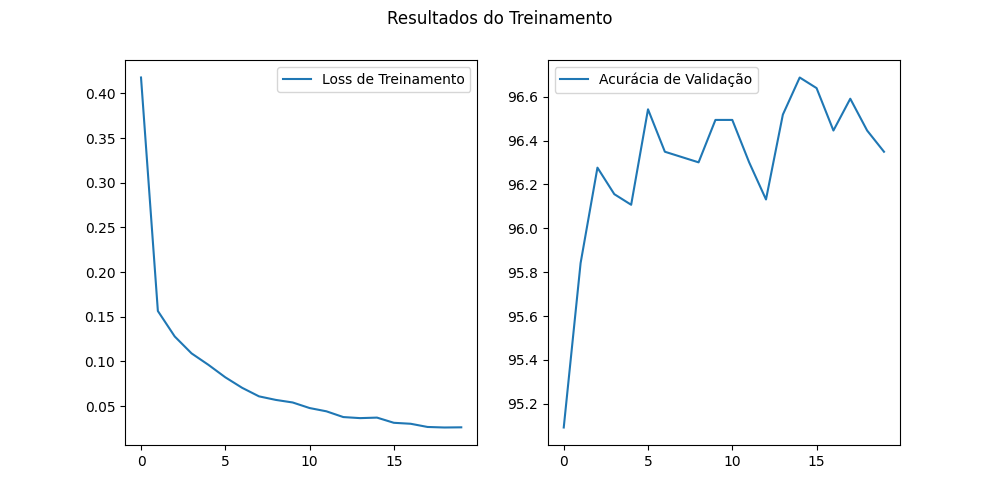
\includegraphics[width=0.8\linewidth]{images/br-numeros.png}
    \caption{Curvas de treinamento do modelo de classificação de números em placas do tipo Brasil}
    \label{fig:brnumerostrain}
\end{figure}

\begin{figure}[H]
    \centering
    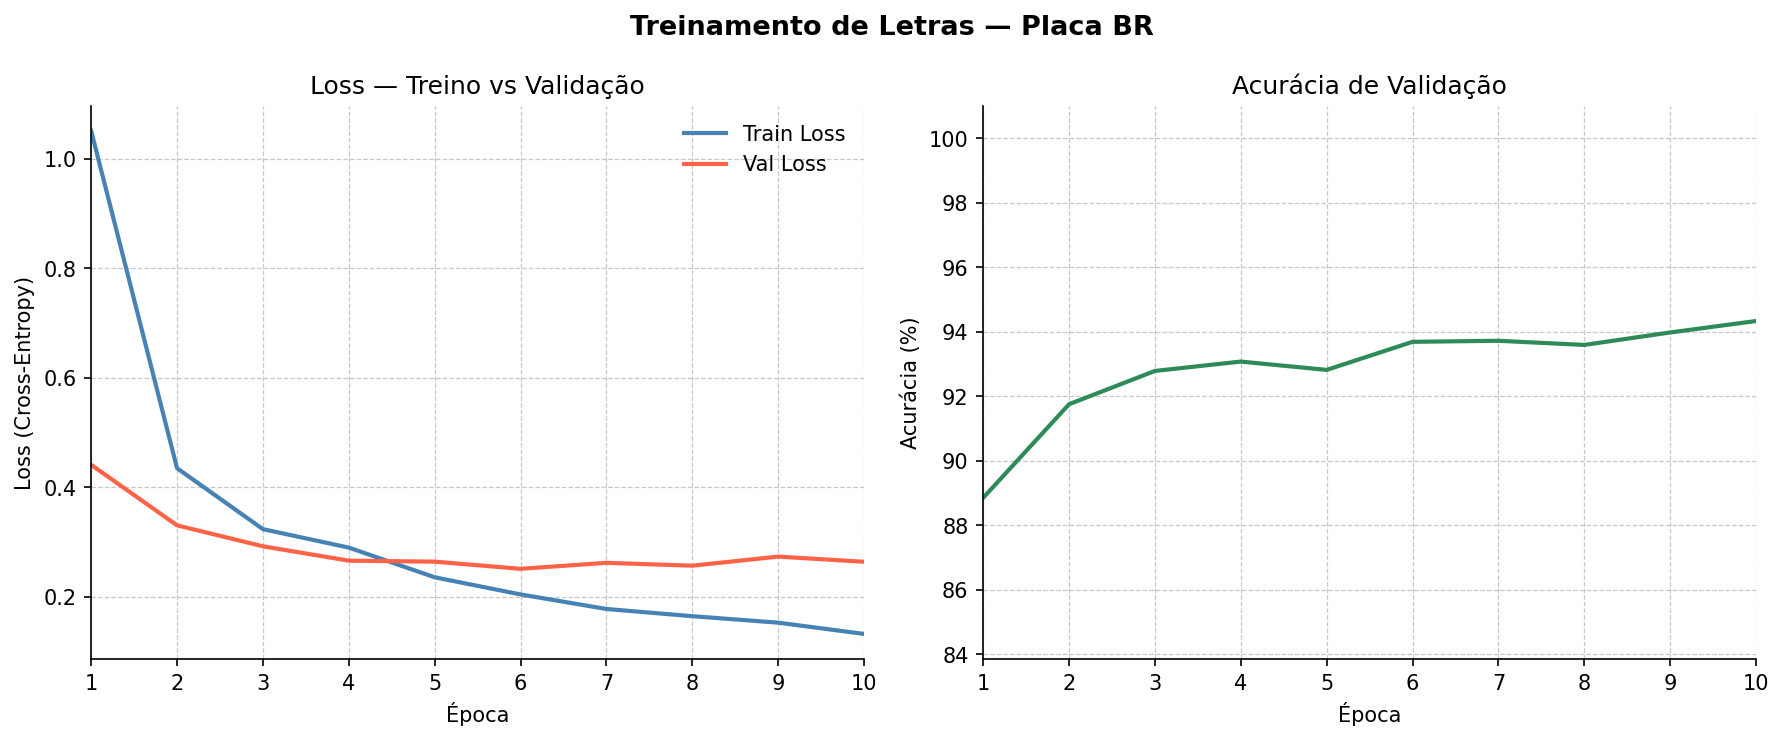
\includegraphics[width=0.8\linewidth]{images/br-letras.png}
    \caption{Curvas de treinamento do modelo de classificação de letras em placas do tipo Brasil}
    \label{fig:brletrastrain}
\end{figure}

\subsection{Extração e classificação simultânea}

O treinamento dos modelos de extração e classificação seguiu um processo parecido. Esse modelo, diferente dos modelos de classificação de caracteres isolados, recebe uma imagem de placa e classifica todos os seus caracteres de uma só vez. O objetivo é que o modelo aprenda a identificar a posição dos caracteres e ao mesmo tempo classificá-los.

Esse modelo, por ser maior e mais complexo, utilizou também algumas técnicas mais refinadas de treinamento. Uma delas foi o \textit{learning rate} variável, que aumenta ou diminui ao longo do treinamento. Outra foi o \textit{early stopping}, que interrompe o treinamento ao identificar que a performance está estagnada.

Os parâmetros de treinamento foram:

\begin{itemize}
    \item \textit{Optimizer}: AdamW com \textit{learning rate} de 0.003 e \textit{weight decay} de 0.004
    \item Tamanho do \textit{batch}: 64
    \item Número de épocas: 100
    \item Paciência: 20
\end{itemize}

A paciência determina a quantidade de épocas que podem ocorrer sem melhoras na acurácia do modelo. Após essa quantidade de épocas sem melhoria o treinamento é interrompido.

Foram treinados dois modelos distintos, um para placas do tipo Brasil e outro para placas do tipo Mercosul. As figuras \ref{fig:train_br} e \ref{fig:train_me} mostram a evolução da \textit{Loss}, da acurácia por caractere e da acurácia por placa ao longo das épocas de treinamento.

\begin{figure}[H]
    \centering
    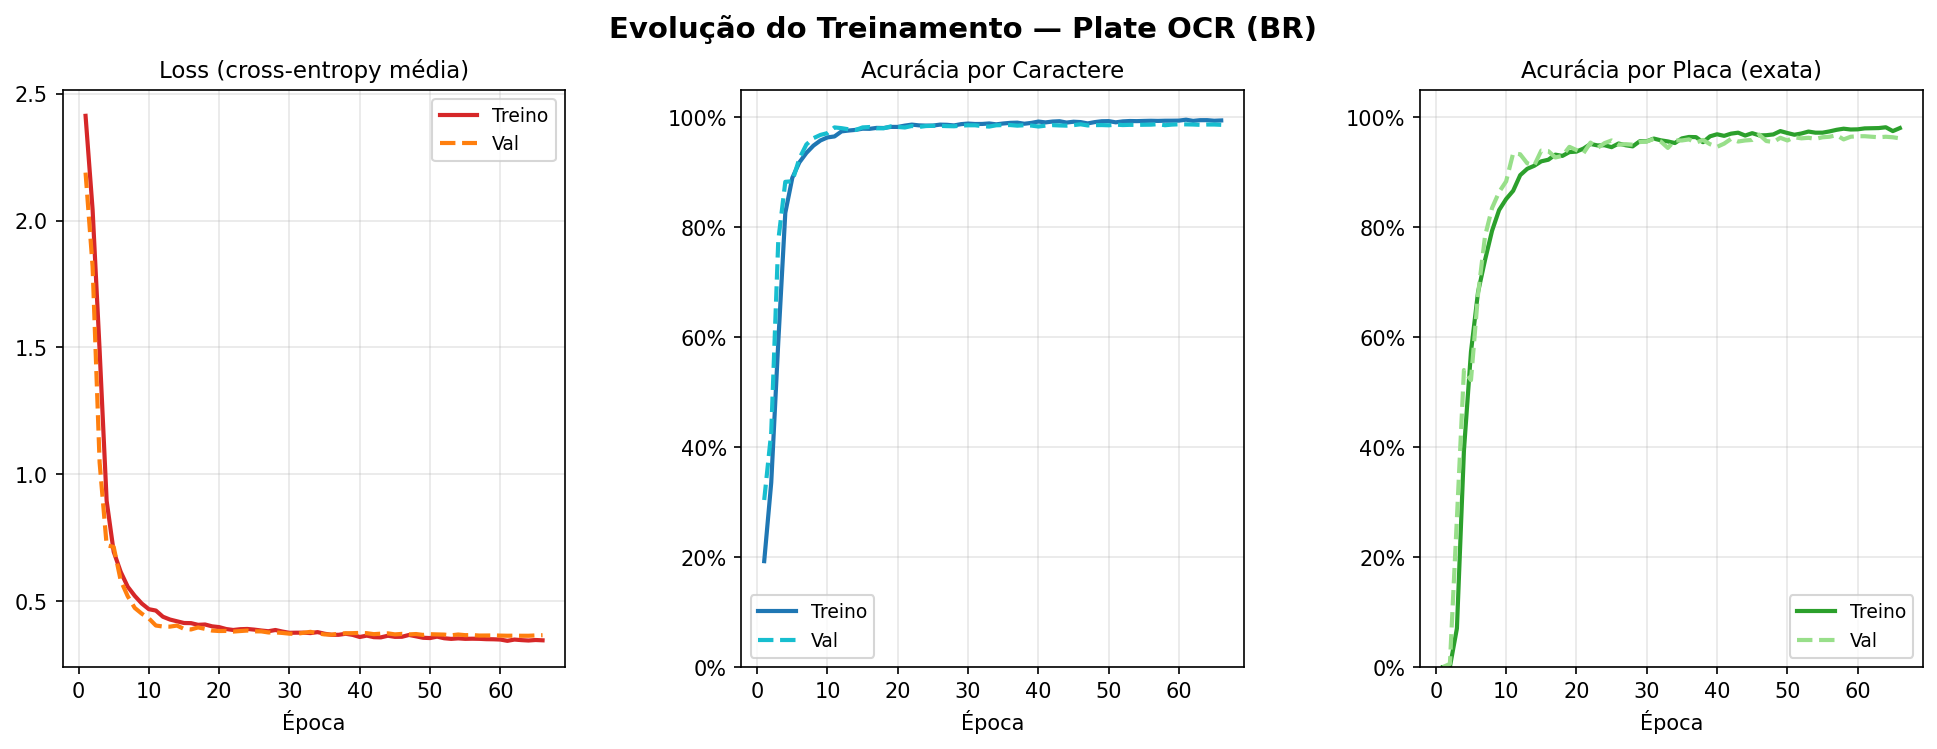
\includegraphics[width=1.0\linewidth]{images/training_curves_br.png}
    \caption{Curvas de treinamento do modelo de classificação em placas do tipo Brasil}
    \label{fig:train_br}
\end{figure}

\begin{figure}[H]
    \centering
    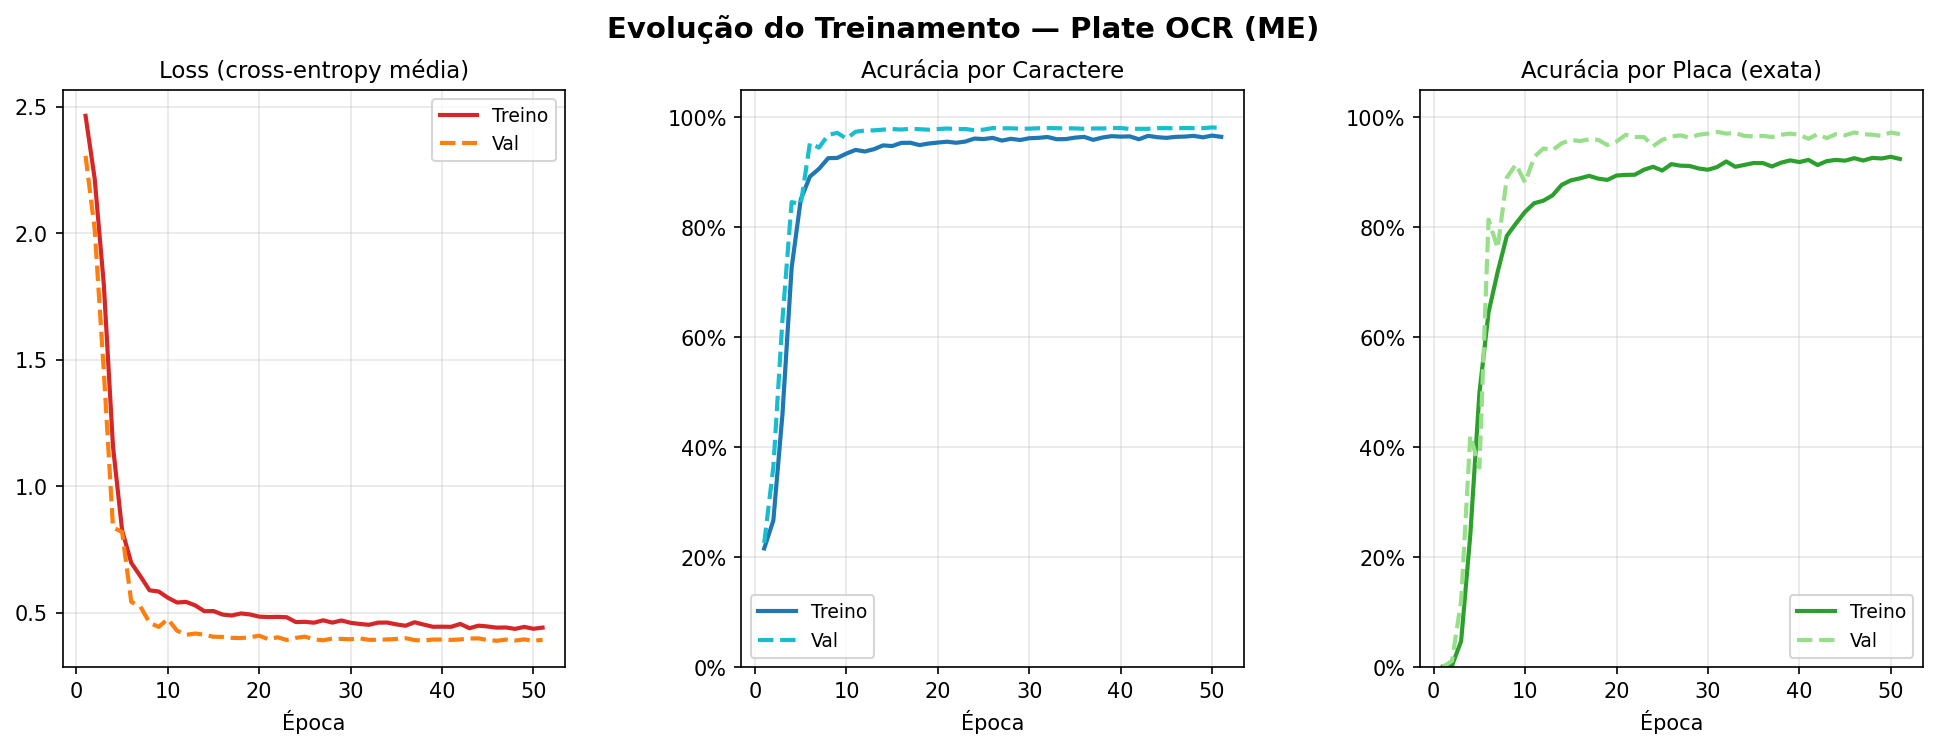
\includegraphics[width=1.0\linewidth]{images/training_curves_me.png}
    \caption{Curvas de treinamento do modelo de classificação em placas do tipo Mercosul}
    \label{fig:train_me}
\end{figure}

\section{Quantização e transformação dos modelos para formato compatível com o \textit{hardware}}

Todos os modelos treinados foram convertidos para o formato ONNX, que pode ser utilizado para execução na placa Rock 3A, porém sem tirar proveito da NPU. Para que a NPU possa ser utilizada, é necessário que os modelos sejam convertidos para o formato RKNN. A Rockchip, fabricante do chip de processamento utilizado na Rock 3A, disponibiliza um \textit{software} na forma de uma biblioteca do python que permite a compilação dos modelos nesse formato. Porém, é necessário que o programa seja executado em um ambiente \textit{linux} da distribuição Ubuntu versão 24.

É possível, no entanto, criar um ambiente com essas condições dentro do \textit{windows} ou outros sistemas operacionais através de um \textit{container} Docker. Um \textit{container} Docker é um ambiente isolado dentro de um computador no qual pode ser instalado \textit{software} sem afetar a máquina que contém o \textit{container}. Esse \textit{container} pode ter qualquer sistema operacional compatível com a máquina, incluindo o Ubuntu 24.

Foi então criado um \textit{container} no qual foi instalado o python e todas as bibliotecas necessárias, incluindo o \textit{rknn toolkit}, responsável pela conversão.

O código de conversão é um \textit{script} simples, que necessita apenas que se aponte para o arquivo ONNX de origem, se preencha algumas informações de configuração e aponte para o \textit{dataset} de quantização, caso se queira quantizar o modelo. A quantização tem potencial de aumentar consideravelmente a performance na NPU, sendo portanto altamente recomendada.

\subsection{Criação dos datasets de quantização}

\section{Preparação do \textit{hardware}}

\section{Testes realizados}